\documentclass{article}
\usepackage{pgf,tikz}
\usetikzlibrary{plotmarks}

\begin{filecontents}{parab.dat}
#x                  y
0        -2
0.5      -0.25
1         1
2         2
3         1 
3.5      -0.25
4        -2
\end{filecontents}

\begin{document}
\pagestyle{empty}

\definecolor{darkgray}{rgb}{0.25,0.25,0.25}
\definecolor{lightgray}{rgb}{0.75,0.75,0.75}

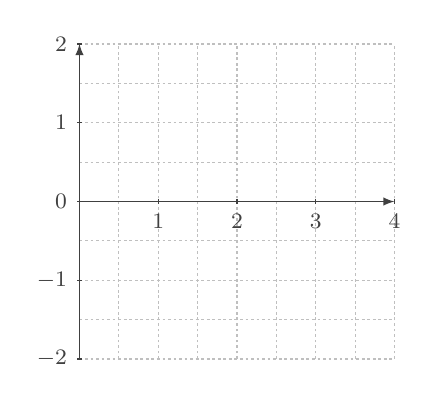
\begin{tikzpicture}[only marks,scale=1]
  \draw [color=lightgray,dash pattern=on 1pt off 1pt, xstep=0.5cm,ystep=0.5cm]
                                                 (0,-2) grid (4,2);
%creating the ticks and xy-axis nodes
  \draw[-latex,color=darkgray,thin] (0,0) -- (4,0);
   \foreach \x in {1,2,3,4}
   \draw[shift={(\x,0)},color=darkgray,thin] (0pt,1pt) -- (0pt,-1pt)
                                   node[below] {\footnotesize $\x$};
   \draw[-latex,color=darkgray] (0,-2) -- (0,2);
      \foreach \y in {-2,-1,0, 1,2}
      \draw[shift={(0,\y)},color=darkgray,thin] (1pt,0pt) -- (-1pt,0pt)
                                    node[left] {\footnotesize $\y$};

%draw the datafile
  \draw plot[mark=*] file {parab.dat};
\end{tikzpicture}



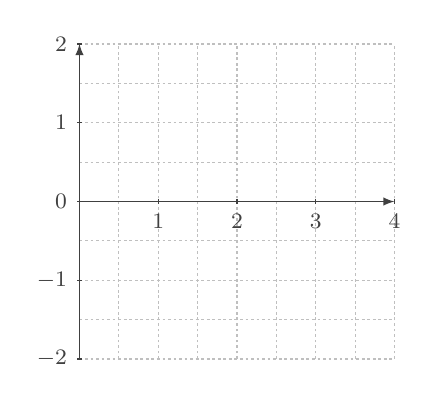
\begin{tikzpicture}[scale=1]
  \draw [color=lightgray,dash pattern=on 1pt off 1pt, xstep=0.5cm,ystep=0.5cm]
                                                 (0,-2) grid (4,2);
%creating the ticks and xy-axis nodes
  \draw[-latex,color=darkgray,thin] (0,0) -- (4,0);
   \foreach \x in {1,2,3,4}
   \draw[shift={(\x,0)},color=darkgray,thin] (0pt,1pt) -- (0pt,-1pt)
                                   node[below] {\footnotesize $\x$};
   \draw[-latex,color=darkgray] (0,-2) -- (0,2);
      \foreach \y in {-2,-1,0, 1,2}
      \draw[shift={(0,\y)},color=darkgray,thin] (1pt,0pt) -- (-1pt,0pt)
                                    node[left] {\footnotesize $\y$};

%draw the datafile
  \draw plot[mark=*] file {parab.dat};
\end{tikzpicture}


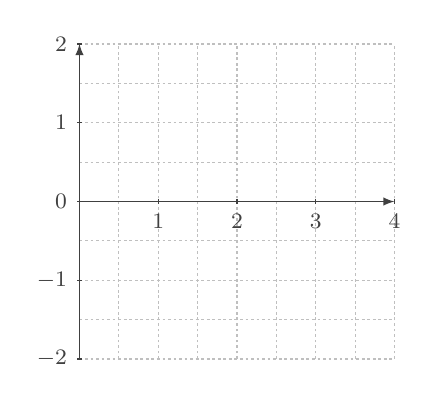
\begin{tikzpicture}[domain=0:4,scale=1]
  \draw [color=lightgray,dash pattern=on 1pt off 1pt, xstep=0.5cm,ystep=0.5cm]
                                                 (0,-2) grid (4,2);
%creating the ticks and xy-axis nodes
  \draw[-latex,color=darkgray,thin] (0,0) -- (4,0);
   \foreach \x in {1,2,3,4}
   \draw[shift={(\x,0)},color=darkgray,thin] (0pt,1pt) -- (0pt,-1pt)
                                   node[below] {\footnotesize $\x$};
   \draw[-latex,color=darkgray] (0,-2) -- (0,2);
      \foreach \y in {-2,-1,0, 1,2}
      \draw[shift={(0,\y)},color=darkgray,thin] (1pt,0pt) -- (-1pt,0pt)
                                    node[left] {\footnotesize $\y$};

%draw the datafile
  \draw plot[mark=*] file {parab.dat};
  \draw [color=blue] plot[id=parab] function {-x**2 +4*x -2};
\end{tikzpicture}


\end{document}
